\documentclass[12pt, oneside]{book}

% toto som navysil!

\usepackage[a4paper,top=3cm,bottom=3.5cm,left=3cm,right=3cm]{geometry}
%\usepackage[a4paper,top=2.5cm,bottom=2.5cm,left=3.5cm,right=2cm]{geometry}

\usepackage[utf8]{inputenc}
\usepackage[T1]{fontenc}
\usepackage{graphicx}
\usepackage{url}
\usepackage{float}
\usepackage{listings,xcolor}
\usepackage[english]{babel} % vypnite pre prace v anglictine
\linespread{1.25} % hodnota 1.25 by mala zodpovedat 1.5 riadkovaniu
\usepackage{xcolor}
\usepackage{textcomp}
\usepackage{inconsolata}
\usepackage[toc,page]{appendix}

\usepackage{todonotes}
%\usepackage[disable]{todonotes}

%%% TODO Notes
\newcommand{\assignment}[2][]{\todo[inline,bordercolor=green!67!yellow!75!black!50,color=green!67!yellow!25,size=\footnotesize,#1]{#2}}
\newcommand{\overview}[2][]{\todo[inline,color=blue!85!green!25,bordercolor=blue!85!green!50!black!50,size=\footnotesize,#1]{#2}}
\newcommand{\minor}[2][]{\todo[color=gray!30,bordercolor=gray,inline,size=\footnotesize,#1]{#2}}
\newcommand{\cutting}[2][]{\todo[color=yellow!30,bordercolor=yellow!50!black!50,inline,size=\footnotesize,#1]{#2}}
\newcommand{\bigassignment}[2][]{\todo[inline, caption={Big assignment},
    color=green!40, #1]{\begin{minipage}{\textwidth-4pt}#2\end{minipage}}}
\newskip\movedskip
\newcommand{\movespaceafter}[1]{%
    \movedskip=0pt%
    \ifhmode\ifdim\lastskip=0pt\else\movedskip=\lastskip\unskip\fi\fi
    #1\ifdim\movedskip=0pt\else\hskip\movedskip\fi
    \ignorespaces}
\newcommand{\reviewnote}[3][]{%
  \movespaceafter{\todo[inline,color=yellow!75!white,linecolor=yellow!85!black,#1]
      {\textsf{\bfseries Review #2:} \ignorespaces#3\par}}%
}
\newcommand{\comment}[3][]{%
  \movespaceafter{\todo[color=green!40,#1]
      {\textsf{\bfseries #2:} \ignorespaces#3\par}}%
}


% Definitions of listings
\definecolor{dkgreen}{rgb}{0.0, 0.42, 0.24}
\definecolor{dkblue}{rgb}{0,0,.6}
\definecolor{dkyellow}{cmyk}{0,0,.8,.3}

\lstset{
  language        = php,
  basicstyle      = \scriptsize\ttfamily,
  keywordstyle    = \color{dkblue},
  stringstyle     = \color{red},
  identifierstyle = \color{dkgreen},
  commentstyle    = \color{gray},
  emph            =[1]{php},
  emphstyle       =[1]\color{black},
  emph            =[2]{if,and,or,else},
  emphstyle       =[2]\color{dkyellow}}

\usepackage{courier}
\lstset{
    basicstyle=\scriptsize\ttfamily,
    numberstyle=\tiny,
    numbersep=5pt,
    tabsize=2,
    extendedchars=true,
    breaklines=true,
    keywordstyle=\color{red},
    frame=b,
    showspaces=false,
    showtabs=false,
    xleftmargin=17pt,
    framexleftmargin=17pt,
    framexrightmargin=5pt,
    framexbottommargin=4pt,
    %showstringspaces=false,
    %escapeinside={}{}
  language        = php,
  keywordstyle    = \color{dkblue},
  stringstyle     = \color{dkyellow},
  identifierstyle = \color{black},
  commentstyle    = \color{gray},
  emph            =[1]{var, const, abstract, 
                        protected, private, public,
                        static, final, extends, implements,
                        global, class, function, try, catch, new},
  emphstyle       =[1]\color{red},
}
\usepackage{caption}
\DeclareCaptionFont{white}{\color{white}}
\DeclareCaptionFormat{listing}{\colorbox[cmyk]{0.43, 0.35, 0.35,0.01}{\parbox{\textwidth}{\hspace{15pt}#1#2#3}}}
\captionsetup[lstlisting]{format=listing,labelfont=white,textfont=white, singlelinecheck=false, margin=0pt, font={bf,footnotesize}}
% end of listings

% -------------------
% --- Definicia zakladnych pojmov
% --- Vyplnte podla vasho zadania
% -------------------
\def\mfrok{Bratislava 2016}
\def\mfnazov{Assignments Workflow in a Learning Management System}
\def\mftyp{Master thesis}
\def\mfautor{Bc. Tomáš Trungel}
\def\mfskolitel{RNDr. Martin Homola, PhD.}

%ak mate konzultanta, odkomentujte aj jeho meno na titulnom liste
\def\mfkonzultant{doc. RNDr. Zuzana Kubincová, PhD.}  

\def\mfmiesto{Bratislava, \mfrok}

%aj cislo odboru je povinne a je podla studijneho odboru autora prace
\def\mfodbor{2511 Applied Informatics} 
\def\program{ Applied Informatics }
\def\mfpracovisko{ Department of Applied Informatics }

\begin{document}     

% -------------------
% --- Obalka ------
% -------------------
\thispagestyle{empty}

\begin{center}
\sc\large
Comenius University in Bratislava\\
Faculty of mathematics, physics and informatics

\vfill

{\LARGE\mfnazov}\\
\mftyp
\end{center}

\vfill

{\sc\large 
\noindent 
\mfrok \hfill \hfill \mfautor
}

\eject % EOP i
% --- koniec obalky ----

% -------------------
% --- Titulný list
% -------------------

\thispagestyle{empty}
\noindent

\begin{center}
\sc  
\large
Comenius University in Bratislava\\
Faculty of mathematics, physics and informatics

\vfill

{\LARGE\mfnazov}\\
\mftyp
\end{center}

\vfill

\noindent
\begin{tabular}{ll}
Study programme: & \program \\
Field of study: & \mfodbor \\
Department: & \mfpracovisko \\
Supervisor: & \mfskolitel \\
Consultant: & \mfkonzultant \\
\end{tabular}

\vfill


\noindent \mfmiesto\\
\mfautor

\eject % EOP i


% --- Koniec titulnej strany


% -------------------
% --- Zadanie z AIS
% -------------------
% v tlačenej verzii s podpismi zainteresovaných osôb.
% v elektronickej verzii sa zverejňuje zadanie bez podpisov

\newpage 
\thispagestyle{empty}
\hspace{-2cm}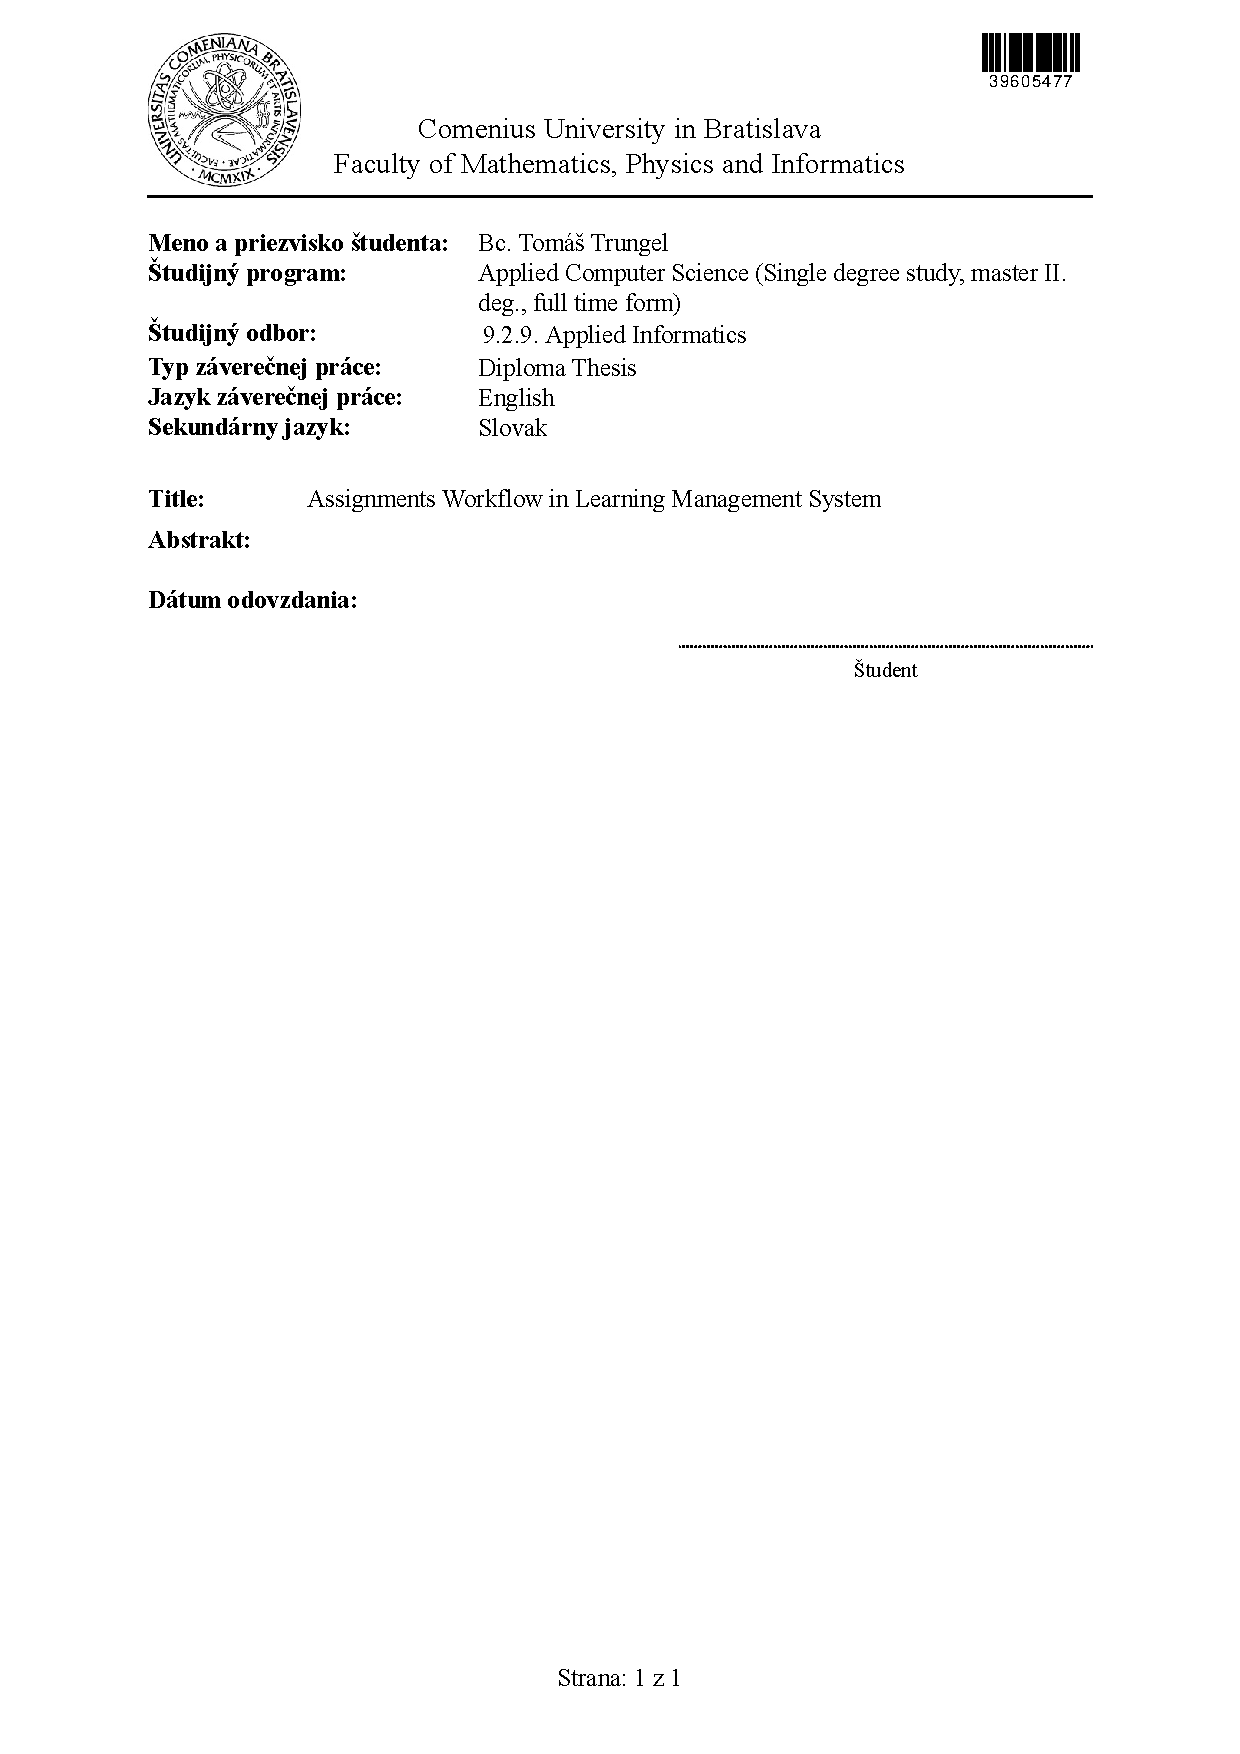
\includegraphics[width=1.1\textwidth]{images/zadanie}

% --- Koniec zadania

% --- Copyright
\newpage

\noindent
\begin{minipage}{0.25\textwidth}~\end{minipage}
\begin{minipage}{0.68\textwidth}
By this I declare that I wrote this master thesis by myself, only with the help of the referenced literature, under the careful supervision of my thesis advisor.
\bigskip\bigskip

\hfill\hbox to 6cm{\dotfill}
\end{minipage}
\vfill\eject % EOP iii
~\vfill\eject % EOP iv


% ---- End copyright

\frontmatter

% -------------------
%   Poďakovanie - nepovinné
% -------------------
\setcounter{page}{3}
\newpage 

\begin{minipage}{0.25\textwidth}~\end{minipage}
\begin{minipage}{0.68\textwidth}
{\bf Acknowledgment:} I would like to say thank You to my master thesis supervisor Martin Homola for his help and professional and valuable advices while I was writing this thesis.\bigskip\bigskip

\end{minipage}
\newpage
% --- Koniec poďakovania


% -------------------
% --- Abstrakt - Anglicky 
% -------------------
\newpage 
\chapter*{Abstract}

Learning management systems are a must at a modern University. One of these systems used at our Faculty is Courses 2, which consits of multiple modules.

In this thesis, we focus on Assignments module. We analyze its weaknesses, then propose and implement improvements and describe the problems that occured during development.

Fist important improvement is added suppport for mirroring assignments, which are in form of web pages. We built an algorithm for recursive downloading of these pages, with added support for logging in of a user and even mirroring of redirect and error HTTP status codes.

Second important improvement are Team Projects with peer review and teamwork review. These concepts aim to teach students constructive critisism, the ability of self\-reflection or job evaluation. We describe its design and implementation.

We also introduce other concepts like Improved Submissions and Assignments Dashboard.





\paragraph*{Keywords:} Learning Management System, Web page Mirroring, Team Projects, Courses 2, Assignments

% --- Koniec Abstrakt - Anglicky

% -------------------
%   Abstrakt - Slovensky
% -------------------
\newpage 
\section*{Abstrakt}


Slovenský abstrakt: TODO

\paragraph*{Kľúčové slová:} jedno, druhé, tretie
% --- Koniec Abstrakt - Slovensky

% -------------------
% --- Predhovor - v informatike sa zvacsa nepouziva
% -------------------
%\newpage 
%\thispagestyle{empty}
%
%\huge{Predhovor}
%\normalsize
%\newline
%Predhovor je všeobecná informácia o práci, obsahuje hlavnú charakteristiku práce 
%a okolnosti jej vzniku. Autor zdôvodní výber témy, stručne informuje o cieľoch 
%a význame práce, spomenie domáci a zahraničný kontext, komu je práca určená, 
%použité metódy, stav poznania; autor stručne charakterizuje svoj prístup a svoje 
%hľadisko. 
%
% --- Koniec Predhovor


% -------------------
% --- Obsah
% -------------------

\newpage 

\tableofcontents
\lstlistoflistings
\listoffigures

% ---  Koniec Obsahu

% -------------------
% --- Zoznamy tabuliek, obrázkov - nepovinne
% -------------------

\newpage 

% TODO: UNCOMMENT
% \listoffigures

% ---  Koniec Zoznamov

\mainmatter


\input introduction.tex 

\part{Background}
\input http.tex
\input mvc.tex
\input codeigniter.tex
\input courses.tex
\part{Implementation}
\input team_projects.tex
\input mirroring.tex
\input peer_review.tex 
\input zaver.tex


% -------------------
% --- Bibliografia
% -------------------


\newpage	

\backmatter

\thispagestyle{empty}
\nocite{*}
\clearpage

\bibliographystyle{plain}
\bibliography{literatura} 


%Prípadne môžete napísať literatúru priamo tu
%\begin{thebibliography}{5}
 
%\bibitem{br1} MOLINA H. G. - ULLMAN J. D. - WIDOM J., 2002, Database Systems, Upper Saddle River : Prentice-Hall, 2002, 1119 s., Pearson International edition, 0-13-098043-9

%\bibitem{br2} MOLINA H. G. - ULLMAN J. D. - WIDOM J., 2000 , Databasse System implementation, New Jersey : Prentice-Hall, 2000, 653s., ???

%\bibitem{br3} ULLMAN J. D. - WIDOM J., 1997, A First Course in Database Systems, New Jersey : Prentice-Hall, 1997, 470s., 

%\bibitem{br4} PREFUSE, 2007, The Prefuse visualization toolkit,  [online] Dostupné na internete: <http://prefuse.org/>

%\bibitem{br5} PREFUSE Forum, Sourceforge - Prefuse Forum,  [online] Dostupné na internete: <http://sourceforge.net/projects/prefuse/>

%\end{thebibliography}

%---koniec Referencii

% -------------------
%--- Prilohy---
% -------------------

%Nepovinná časť prílohy obsahuje materiály, ktoré neboli zaradené priamo  do textu. Každá príloha sa začína na novej strane.
%Zoznam príloh je súčasťou obsahu.
%
%\addcontentsline{toc}{chapter}{Appendix A}
%\input appendixA.tex
%
%\addcontentsline{toc}{chapter}{Appendix B}
%\input AppendixB.tex
\begin{appendices}
\input appendixA.tex
\input appendixB.tex
\end{appendices}

\end{document}






